% Compile: pdflatex diagram-wham.tex && dvisvgm --pdf --no-fonts diagram-wham.pdf
\documentclass[border=12pt]{standalone}
\usepackage{tikz}
\usetikzlibrary{arrows.meta, positioning, decorations.pathreplacing}
\usepackage[sfdefault]{carlito}
\definecolor{card}{HTML}{FFFFFF}
\definecolor{ink}{HTML}{0F1730}
\definecolor{cyanA}{HTML}{0E7490}
\definecolor{violetA}{HTML}{6D28D9}
\definecolor{emeraldA}{HTML}{047857}
\begin{document}
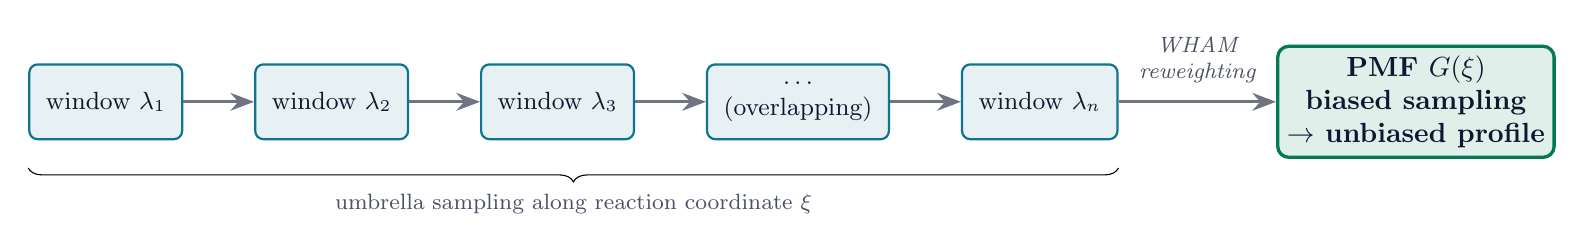
\begin{tikzpicture}[
  font=\small,
  win/.style={draw=cyanA, thick, rounded corners=3pt, fill=cyanA!10, text=ink,
           align=center, minimum height=0.95cm, inner sep=6pt},
  pmf/.style={draw=emeraldA, very thick, rounded corners=4pt, fill=emeraldA!12, text=ink,
           align=center, minimum height=1.2cm, font=\bfseries},
  arr/.style={-{Stealth[length=3mm]}, very thick, color=ink!60},
  lab/.style={font=\footnotesize\itshape, text=ink!75, align=center}
]
  \node[win] (W1) {window $\lambda_1$};
  \node[win] (W2) [right=0.9cm of W1] {window $\lambda_2$};
  \node[win] (W3) [right=0.9cm of W2] {window $\lambda_3$};
  \node[win] (W4) [right=0.9cm of W3] {$\dots$\\ (overlapping)};
  \node[win] (W5) [right=0.9cm of W4] {window $\lambda_n$};
  \node[pmf] (PMF) [right=2.0cm of W5] {PMF $G(\xi)$\\ biased sampling\\ $\to$ unbiased profile};

  \draw[arr] (W1) -- (W2);
  \draw[arr] (W2) -- (W3);
  \draw[arr] (W3) -- (W4);
  \draw[arr] (W4) -- (W5);
  \draw[arr] (W5) -- (PMF) node[lab, midway, above=3pt] {WHAM\\ reweighting};

  \draw[decorate, decoration={brace, amplitude=5pt, mirror}] ([yshift=-10pt]W1.south west) -- node[below=6pt, font=\footnotesize, text=ink!75] {umbrella sampling along reaction coordinate $\xi$} ([yshift=-10pt]W5.south east);
\end{tikzpicture}
\end{document}